\documentclass[dvisvgm,hypertex,aspectratio=169]{beamer}
\usefonttheme{serif}

%\usepackage[utf8]{inputenc}
%\usepackage[T1]{fontenc}

%\usepackage[draft]{animate}
\usepackage[final]{animate}
\usepackage{ifthen}


%\usepackage{pythontex} % <--
\usepackage{graphicx}


\usepackage{tikz}
\usepackage{pgfplots}
\usepackage{pgfplotstable}
\pgfplotsset{compat=1.16}
\usetikzlibrary{calc}
\usetikzlibrary{decorations.pathmorphing,patterns}
\usepackage{amsmath}


%%%%%%%%%%%%%%%%%%%%%%%%%%%%%%%%%%%%%%%%%%%%%%%%%%%%%%%%%%%%%%%%%%%%%%%%%%%%%%% 
% Define footer
\usepackage{ccicons}

\makeatletter
\setbeamertemplate{footline}
{
  \leavevmode%
  \hbox{%
  %\begin{beamercolorbox}[wd=.333333\paperwidth,ht=2.25ex,dp=1ex,center]{title in head/foot}%
    %\usebeamerfont{title in head/foot}\insertsubsection
  %\end{beamercolorbox}%
  %\begin{beamercolorbox}[wd=.333333\paperwidth,ht=2.25ex,dp=1ex,right]{date in head/foot}%
  %  \usebeamerfont{date in head/foot}\insertshortdate{}\hspace*{2em}
  %  \insertframenumber{} / \inserttotalframenumber\hspace*{2ex} 
  %\end{beamercolorbox}}%
  %\vskip0pt%
  \begin{beamercolorbox}[wd=.92\paperwidth,ht=2.25ex,dp=1ex,right]{author in head/foot}%
    \usebeamerfont{author in head/foot}\insertauthor
  \end{beamercolorbox}%
  \begin{beamercolorbox}[wd=.08\paperwidth,ht=2.25ex,dp=1ex,right]{date in head/foot}%
    \ccbysa
  \end{beamercolorbox}}%
  \vskip0pt%
}
\makeatother
%%%%%%%%%%%%%%%%%%%%%%%%%%%%%%%%%%%%%%%%%%%%%%%%%%%%%%%%%%%%%%%%%%%%%%%%%%%%%%%


\author{\href{mailto:kjartan@tec.mx}{kjartan@tec.mx}}

\begin{document}

\section{Create animation}

\IfFileExists{./bode-example.dta}{%
  \pgfplotstableread[col sep=comma]{bode-example.dta}{\btable}

  \def\tend{20}
\begin{frame}[label=A]{Sinusoid in - sinusoid out}
      \begin{center}
        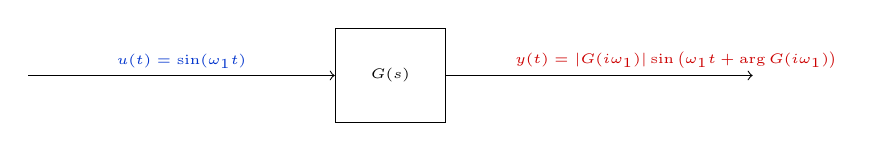
\begin{tikzpicture}[scale=0.6]
          \tiny
          \node[draw, minimum width=14mm, minimum height=12mm] (sys) {$G(s)$};
          \node[coordinate, left of=sys, node distance=46mm] (input) {};
          \node[coordinate, right of=sys, node distance=46mm] (output) {};
          \draw[->] (input) -- node[ above] {$\textcolor{blue!80!green}{u(t)=\sin(\omega_1 t)}$} (sys);
          \draw[->] (sys) -- node[near end, above] {$\textcolor{red!80!black}{y(t)=|G(i\omega_1)|\sin\big(\omega_1 t + \arg G(i\omega_1)\big)}$} (output);
        \end{tikzpicture}
      \end{center}
      \begin{center}
        \begin{animateinline}[controls, loop, palindrome]{4}
          \multiframe{36}{n=0+1}{
            \pgfplotstablegetelem{\n}{0}\of\btable
            \pgfmathsetmacro{\ww}{\pgfplotsretval}
            \pgfplotstablegetelem{\n}{1}\of\btable
            \pgfmathsetmacro{\gain}{\pgfplotsretval}
            \pgfplotstablegetelem{\n}{2}\of\btable
            \pgfmathsetmacro{\phshift}{\pgfplotsretval}
            \pgfmathsetmacro{\nsamples}{\ww*30}

            \begin{tikzpicture}[scale=0.5, transform shape]

              \begin{loglogaxis} [
            width=7cm,
            height=5cm,
            ylabel=$|G|$,
            %xticklabels=\empty,
            ytick={10, 1, 0.1, 0.01, 0.001, 0.0001, 0.0001, 0.00001},
            grid=both,
            minor y tick num=9,
            % extra y ticks={.5}, % how to convert to fixed point tick label ?
            % extra y tick style={log identify minor tick positions=true},
            every major grid/.style={red, opacity=0.5},
            ymin=0.01, ymax=10,
            ]
            \addplot+[thick, black, no marks,] table[x index=0, y index=1] {\btable};
            \draw[thick, blue!80!green] (axis cs: \ww, 0.01) -- (axis cs: \ww, 10);
          \end{loglogaxis}
          \begin{semilogxaxis} [
            xlabel=$\omega$,
            ylabel=$\arg G$,
            xshift = 7cm, 
            width=7cm,
            height=5cm,
            grid=both,
            ytick={0, -90, -180},
            minor y tick num=2,
            every major grid/.style={red, opacity=0.5},
            %legend entries={Bessel filter, Delay of one},
            %legend pos={south west},
            ]
            \addplot+[thick, black, no marks,] table[x index=0, y index=2] {\btable};
            \draw[thick, blue!80!green] (axis cs: \ww, -190) -- (axis cs: \ww, 10);
          \end{semilogxaxis}
          \begin{axis} [
            width = 12cm,
            height=5cm,
            yshift = -6cm,
            xlabel = {$t$},
            ymin=-3.2,
            ymax = 3.2,
            ]
            \addplot+[thick, blue!80!green, no marks, domain=0:\tend, samples=\nsamples, smooth] {sin(\ww*180/3.14*x)};
            \addplot+[thick, red!80!black, no marks, domain=0:\tend, samples=\nsamples, smooth] {\gain*sin(\ww*180/3.14*x + \phshift)};
            
          \end{axis}
        \end{tikzpicture}
      }
    \end{animateinline}
  \end{center}
\end{frame}
}{}
\end{document}


